% 05-results.tex -- results of the main run (540 runs, 17/11) and of the energy run
% with KVM halt-polling disabled (108 runs, 18/11). Numbers are medians across
% repetitions; tables are generated by analysis/*.py.

\section{RQ1: What Does Each Mesh Cost?}
\label{sec:rq1}

\paragraph{Throughput}
\Cref{tab:sat} reports the maximum throughput each configuration sustains
within the SLO. Every mesh reduces it, but by very different amounts. Ambient
L4 keeps 78--82\% of the no-mesh throughput, the most of any mesh with workload
mTLS. At the other end, CI sustains only 22\% on the echo benchmark, and
the Istio sidecar 30\%. On HR, the waypoint (69\%) and Linkerd (64\%)
keep more than the Istio sidecar (52\%) and CI (49\%). Cilium without L7
rules keeps 82--87\%, more than Ambient L4 on echo (87 against 78\%) and
within the search-to-search spread on OB and HR. Searches that observed a
failing rate differ by up to about 10\% (the wider ranges in \cref{tab:sat}
include bisections that gave only a lower bound), so smaller differences,
such as Linkerd against the Istio sidecar on OB, are not meaningful.

\begin{table}[t]
  \centering
  \caption{Maximum SLO-compliant throughput (req/s) and fraction of the
           no-mesh baseline: median of the searches whose boundary was
           observed, with the range over all searches of the cell (2--3
           searches, \cref{sec:load}).}
  \label{tab:sat}
  \footnotesize
  \setlength{\tabcolsep}{3pt}
  % generated by analysis/13_saturacao.py
\begin{tabular}{@{}lrrr@{}}
\toprule
     & Echo & OB & HR \\
\midrule
B & 14899\,\scriptsize[14012--14899] & 1274 & 2374\,\scriptsize[2287--2431] \\
IA4 & 11688\,\scriptsize[10019--11688] (78\%) & 1003\,\scriptsize[990--1003] (79\%) & 1953 (82\%) \\
CI4 & 12987 (87\%) & 1049 (82\%) & 1981\,\scriptsize[1930--2032] (83\%) \\
IA7 & 8260\,\scriptsize[8208--8312] (55\%) & 953\,\scriptsize[905--953] (75\%) & 1632\,\scriptsize[1067--1671] (69\%) \\
LK & 5726\,\scriptsize[5253--5865] (38\%) & 734\,\scriptsize[715--793] (58\%) & 1518\,\scriptsize[1068--1518] (64\%) \\
IS & 4474\,\scriptsize[4202--4691] (30\%) & 778\,\scriptsize[753--803] (61\%) & 1233 (52\%) \\
CI & 3281\,\scriptsize[2939--3281] (22\%) & 915 (72\%) & 1163\,\scriptsize[1067--1191] (49\%) \\
\bottomrule
\end{tabular}

\end{table}

\paragraph{Tail latency}
\Cref{fig:p99load} shows p99 latency against load, and \cref{tab:p99} the
medians with significance against the baseline. At 90\% load, among the
meshes that authenticate workloads, Ambient L4 adds the least: +60\% on echo,
+62\% on OB, and +54\% on HR. Cilium without L7 rules (CI4, 5 runs per cell)
adds less on HR (+25\%), about the same on OB (+55\%; not significantly
different from Ambient L4 at 30\% and 90\% load), and more on echo in this
run (+128\%), where WireGuard on the single cross-node hop is its whole cost.
A same-day control of B, IA4, CI4, and IS on OB and HR (3 runs each, a week
after the main run) confirms the OB and HR comparisons: CI4 and IA4 have the
same p99 on OB (22.1 against 22.1\,ms at 90\% load), and on HR every CI4 run
was faster than every IA4 run (10.8 against 13.2\,ms).
CI4's echo p99 varies between days more than any other measurement, however:
a control run on a later day, together with CI, gave 1.7--1.8\,ms instead of
2.8--3.0\,ms
(\cref{sec:threats}), so its comparison with Ambient L4 on echo is
inconclusive. The Istio sidecar is
the worst on OB, the application with the deepest call graph (11 internal calls
per request, 10.4 of them across nodes; \cref{sec:rq3}), where its p99 grows by
+1025\% (11.9 to 133.7\,ms). CI is the worst on echo (+799\%), even though
the echo chain has a single internal hop. Linkerd has a lower p99 than the
Istio sidecar in 8 of the 9 cells (+463\% vs.\ +1025\% on OB at 90\% load;
the exception is echo at 30\%, 2.51 vs.\ 2.46\,ms), although both place a
proxy in every pod. The ranking is the same at 60\% load except on echo, where
LK, CI4, IS, and IA7 lie within 0.4\,ms of each other and change order (IA7
and IS are not significantly different). The p99.9 follows it: at 90\% load the
Istio sidecar multiplies the baseline p99.9 by 8.4 on OB and Linkerd by 5.4,
while Ambient L4 stays within 1.2--1.6$\times$ on all three applications;
CI reaches 6.8$\times$ on echo, against 1.5$\times$ for CI4.
The ranking is also reproducible across deployments: in the second run used
for energy (a fresh deployment of every configuration with KVM halt-polling
disabled, 3 repetitions, 30\% and 90\% load), Kendall's $\tau$ between the two p99 rankings is 1.0 in 5 of the
6 application and load cells and 0.87 on HR at 90\%.
Kruskal--Wallis rejects equal p99 across configurations for every application
and load (largest $p = 1.8\times10^{-10}$), all 54 mesh-versus-baseline
comparisons remain significant after Holm correction within each application
and load (largest adjusted $p = 0.0011$), and Cliff's
$\delta = 1$ in every case: every repetition of every mesh is slower than every
repetition of the baseline. Most of the L7 meshes' overhead at 90\% load is load-dependent: on
OB and HR, the increase already present at 30\% load is only 18--39\% of the
increase at 90\% for IS, IA7, LK, and CI, against 44--77\% for IA4 and CI4,
whose overhead is mostly a fixed per-request cost.

\begin{figure}[t]
  \centering
  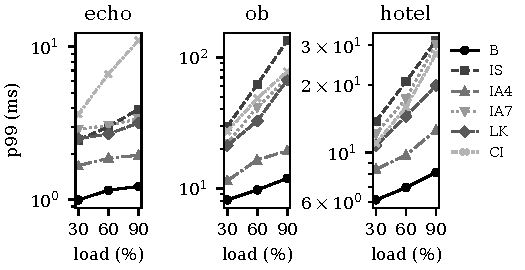
\includegraphics[width=\columnwidth]{figs/p99_carga.pdf}
  \caption{p99 latency vs.\ load level (median of 10 runs; 5 for CI4, run on a
           later day; bands:
           95\% bootstrap confidence interval of the median). Load levels are
           fixed rates, 30/60/90\% of the lowest initial saturation
           estimate (\cref{sec:load}).}
  \label{fig:p99load}
\end{figure}

\begin{table*}[t]
  \centering
  \caption{p99 latency (ms), median of 10 runs (5 for CI4, run on a later day). $^{*}$: different from B
           (Mann--Whitney, Holm-corrected within each column, $p<0.05$).}
  \label{tab:p99}
  \small
  % generated by analysis/20_estatistica.py; do not edit by hand
\begin{tabular}{lrrrrrrrrr}
\toprule
Config. & Echo 30\% & Echo 60\% & Echo 90\% & OB 30\% & OB 60\% & OB 90\% & HR 30\% & HR 60\% & HR 90\% \\
\midrule
B & 1.00 & 1.15 & 1.22 & 8.14 & 9.70 & 11.88 & 6.14 & 6.97 & 8.14 \\
IS & 2.46$^{*}$ & 3.00$^{*}$ & 3.91$^{*}$ & 29.58$^{*}$ & 61.73$^{*}$ & 133.70$^{*}$ & 13.76$^{*}$ & 20.67$^{*}$ & 31.46$^{*}$ \\
IA4 & 1.67$^{*}$ & 1.87$^{*}$ & 1.95$^{*}$ & 11.40$^{*}$ & 16.44$^{*}$ & 19.30$^{*}$ & 8.39$^{*}$ & 9.74$^{*}$ & 12.54$^{*}$ \\
IA7 & 2.88$^{*}$ & 3.07$^{*}$ & 3.38$^{*}$ & 21.95$^{*}$ & 41.51$^{*}$ & 69.31$^{*}$ & 12.11$^{*}$ & 17.35$^{*}$ & 30.35$^{*}$ \\
LK & 2.51$^{*}$ & 2.69$^{*}$ & 3.17$^{*}$ & 21.10$^{*}$ & 32.56$^{*}$ & 66.88$^{*}$ & 10.73$^{*}$ & 14.49$^{*}$ & 19.88$^{*}$ \\
CI & 3.63$^{*}$ & 6.64$^{*}$ & 10.97$^{*}$ & 27.16$^{*}$ & 48.39$^{*}$ & 77.48$^{*}$ & 10.96$^{*}$ & 15.91$^{*}$ & 27.40$^{*}$ \\
CI4 & 3.03$^{*}$ & 2.99$^{*}$ & 2.78$^{*}$ & 11.92$^{*}$ & 14.33$^{*}$ & 18.37$^{*}$ & 7.72$^{*}$ & 8.54$^{*}$ & 10.20$^{*}$ \\
\bottomrule
\end{tabular}
% p99_ms: median of 10 runs (5 for CI4); * = different from B (Mann-Whitney, Holm within each column, p<0.05)

\end{table*}

\paragraph{CPU and memory}
\Cref{fig:resources} breaks CPU down by component, normalized per
1{,}000\,req/s. At 90\% load, among meshes with workload mTLS, Ambient L4 adds
the least CPU (+33\% to +61\% depending on the application), while CI adds the
most on echo and OB (+93\% on OB and
+306\% on echo). The Istio sidecar adds +215\% on echo and +116\% on HR.
On OB at 60\% load, the setting used in the abstract, the extra CPU over
the baseline is 2.6 (IA4), 4.1 (IA7), 4.5 (LK), 6.7 (IS), and 7.0 (CI) cores
per 1{,}000\,req/s. Container CPU misses kernel work done outside any
container, such as WireGuard's encryption in softirq context: CI4's container
CPU is within 7\% of the baseline's at 90\% load and within 13\% at any load. Counting all busy CPU in the four VMs
instead, at the same setting the meshes add 2.0 (CI4), 3.0 (IA4), 4.6 (IA7),
5.2 (LK), 7.5 (IS), and 9.1 (CI) cores per 1{,}000\,req/s, in the same order
as container CPU for the other meshes; in the same-day control, CI4 adds 2.0
and IA4 2.5. Per-request CPU falls with load in every
configuration, most for the L7 proxies (IS's sidecars on OB: 8.1, 6.7, and 4.8
cores per 1{,}000\,req/s at 30, 60, and 90\% load), consistent with more
requests handled per wakeup as queues build; at 90\% load the application
containers under IS and IA7 also use less CPU per request than in the baseline
(3.8 and 4.2 against 5.0), which we have not explained. Relative CPU overheads
are therefore smaller at 90\% than at 60\% load. The dominant component differs by design (OB, 90\% load): the per-pod proxies for the Istio
sidecar and Linkerd (on OB, 4.8 and 3.6 cores per 1{,}000\,req/s), ztunnel
for Ambient L4 (2.1), ztunnel and the waypoint in similar shares for IA7 (1.3
and 1.9), and, for Cilium, the agent and the per-node Envoy in equal parts (2.6
and 3.1). Memory is mostly a fixed cost: the Istio sidecars hold 1.8\,GiB
across the 32 application pods (about 57\,MiB each), against 0.21\,GiB for
Linkerd's proxies (about 7\,MiB each); ztunnel uses about 100\,MiB in total and
the three waypoints 375\,MiB. On the control-plane node, istiod uses 85\,MiB
with sidecars and 155\,MiB in ambient mode, and Linkerd's control plane
140\,MiB. With Istio sidecars, Prometheus also holds about 0.9\,GiB more,
because it scrapes the metrics of every sidecar; we count it as monitoring,
not as mesh cost.

\begin{figure}[t]
  \centering
  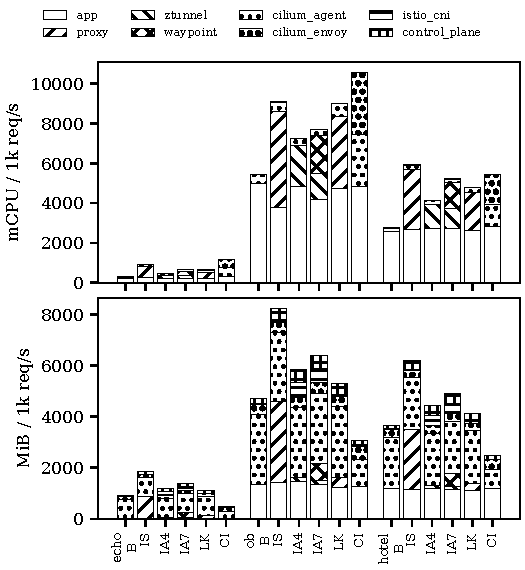
\includegraphics[width=\columnwidth]{figs/recursos.pdf}
  \caption{Container CPU and memory per 1{,}000\,req/s by component, at 90\%
           load (5 runs for CI4, on a later day; its WireGuard work runs in the kernel and
           is not attributed to any container).}
  \label{fig:resources}
\end{figure}

\paragraph{Energy}
\Cref{tab:energy} reports package energy per request, net of the no-mesh idle
power, from a separate run with KVM halt-polling disabled (\cref{sec:design,sec:threats}). Every mesh costs energy, and the ranking mostly follows CPU. At
90\% load, Ambient L4 adds 19--62\% per request (the waypoint is marginally
lower on OB, +16\%), the Istio sidecar 22--129\%,
and Cilium the most, 49--188\%, with its largest overhead on echo. Relative
overheads are lower on OB, where the application itself dominates the energy
per request, and higher at 30\% load, where fixed costs are spread over fewer
requests. With no load, the meshes draw 0.3 (Cilium) to 1.6\,W (Istio sidecar)
above the baseline's 21.0\,W, the sidecar paying for one idle proxy per pod. We did not measure the energy of CI4.

\begin{table}[t]
  \centering
  \caption{Package energy per request (mJ), net of the no-mesh idle power,
           with KVM halt-polling disabled (median of 3 runs).}
  \label{tab:energy}
  \footnotesize
  \setlength{\tabcolsep}{2.5pt}
  % generated by analysis/60_energia.py
\begin{tabular}{lrrrrrr}
\toprule
Config. & Echo 30\% & Echo 90\% & OB 30\% & OB 90\% & HR 30\% & HR 90\% \\
\midrule
B & 4.1 & 2.9 & 48.5 & 36.8 & 19.8 & 16.7 \\
IS & 10.0 & 6.6 & 84.7 & 44.8 & 40.6 & 28.7 \\
IA4 & 6.5 & 4.6 & 67.2 & 43.9 & 30.5 & 23.6 \\
IA7 & 8.1 & 5.7 & 79.3 & 42.8 & 40.1 & 29.1 \\
LK & 8.1 & 5.5 & 78.5 & 49.0 & 35.6 & 26.6 \\
CI & 11.6 & 8.2 & 94.0 & 55.0 & 38.8 & 29.2 \\
\bottomrule
\end{tabular}
% mJ per request, net of the idle power of B, halt_poll_ns = 0

\end{table}

\paragraph{Variability}
Results are stable across repetitions: the coefficient of variation of p99
never exceeds 0.22 (Linkerd on OB at 90\% load). Five of the 540 runs, all on
HR, had error rates between 0.13\% and 0.38\%, and one dropped 37 requests;
all are below the 1\% threshold and are kept.

\section{RQ2: Where Does the Cost Come From?}
\label{sec:rq2}

We profiled every configuration at 60\% load on echo and OB
(\cref{sec:design}) and attribute to the data plane all samples of the proxy
processes (Envoy, \texttt{linkerd2-proxy}, ztunnel, the Cilium agent) plus any
kernel stack that runs WireGuard or an eBPF program. \Cref{fig:perfil}
breaks this CPU down per request and \cref{tab:perfil} summarizes it.

\paragraph{What each data plane spends}
On OB, the baseline spends 0.64\,ms of CPU per request in its data plane (the
Cilium agent and the CNI's eBPF programs, which every configuration also
runs; the increase of a mesh is its total minus this). The Istio sidecar spends 5.5\,ms, of which 61\% is
HTTP/2 framing and header compression (\texttt{nghttp2}): with 11 internal
calls per request, each crossing two sidecars, protocol processing dominates,
as MeshInsight found for an older Envoy~\cite{zhu2023meshinsight}. Ambient L4
spends 2.6\,ms, almost half of it (47\%) in TLS inside ztunnel and no L7
parsing; adding the waypoint (IA7) raises it to 4.2\,ms, split between the
waypoint's HTTP processing (39\%) and ztunnel's TLS (31\%). Linkerd spends
4.6\,ms; because its proxy is distributed without symbols, 46\% of it can only
be attributed to the proxy as a whole, and 13\% is kernel networking. Every
mesh also multiplies kernel crossings: on OB, the data-plane processes (the
proxies and the Cilium agent) make 191 (IS) to 329 (CI) system calls and 58 to
152 context switches per request, against 48 and 31 for the Cilium agent alone
in the baseline.

\paragraph{Why Cilium is the slowest on echo}
On echo, Cilium spends 0.92\,ms of data-plane CPU per request, 9.6$\times$ the
baseline and 1.6$\times$ the Istio sidecar, although the request crosses a
single internal hop. Every request is redirected to the per-node Envoy by the
L7 rule on both nodes, is encrypted by WireGuard (14\% of the total), and makes
the Cilium agent spend almost as much CPU as Envoy itself (36\,s against 39\,s
over the profiling window). It also has the most context switches per request
(27, against 12 for the sidecar). We could not resolve the agent's symbols, so
we located the agent's cost with ablations, run together with a same-day
control of CI (echo, 3 runs each). With Hubble, Cilium's flow observability,
disabled, the agent's CPU at 90\% load falls from 0.96 to 0.36 cores and p99
from 14.4 to 6.7\,ms (8.2 to 4.7\,ms at 60\%): Hubble accounts for 43--54\%
of CI's p99, and every run without it was faster than every run with it. Also
disabling Envoy's access log changes neither. Removing the L7 rule while
keeping WireGuard (CI4) brings p99 down to 1.7\,ms on the same day. The eBPF programs themselves are cheap: with
\texttt{kernel.bpf\_stats\_enabled}, all of Cilium's programs together run
for 40\,\textmu s per echo request and 354\,\textmu s per OB request, 4--5\%
of its data-plane CPU, and the difference to CI4 (19 and 88\,\textmu s) comes
mostly from the program that handles traffic returning from the node's Envoy
(\texttt{cil\_from\_host}). Cilium's overhead therefore comes from redirecting
traffic to the per-node Envoy and from logging every L7 flow to Hubble, not from
its eBPF datapath.

\paragraph{Why the Istio sidecar is the slowest on OB}
On OB, Cilium spends even more CPU per request than the sidecar (7.2 against
5.5\,ms; cAdvisor gives the same order, 7.0 against 6.7 extra cores per
1{,}000\,req/s, \cref{sec:rq1}), yet its p99 is lower (77 against 134\,ms at 90\% load). The
difference is where the work runs. The sidecar's cost follows the frontend,
which issues 10 of the 11 internal calls per request through its own proxy:
that one sidecar uses 1.1--1.3 cores at 90\% load with two worker threads,
while Cilium's per-node Envoys split the L7 work among the nodes that receive
the calls (at most 0.7 cores each). Isolating the frontend on its own node does
not change this, and does not reduce the sidecar's p99 (\cref{sec:rq3}).

\begin{figure}[t]
  \centering
  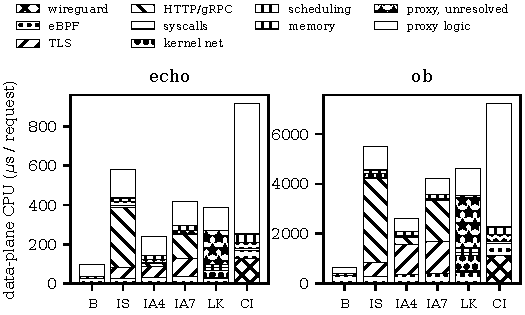
\includegraphics[width=\columnwidth]{figs/perfil.pdf}
  \caption{Data-plane CPU per request by category, at 60\% load (sum of the
           three workers).}
  \label{fig:perfil}
\end{figure}

\begin{table}[t]
  \centering
  \caption{Data-plane CPU per request at 60\% load, share spent in
           cryptography (TLS and WireGuard) and HTTP/gRPC processing, and
           context switches (cs) and system calls (sys) per request of the
           data-plane processes (proxies and the Cilium agent; only the agent
           in B). LK: proxy without symbols, so its TLS and HTTP shares cannot
           be separated.}
  \label{tab:perfil}
  \small
  \setlength{\tabcolsep}{3pt}
  % generated by analysis/50_perfil.py
\begin{tabular}{llrrrrr}
\toprule
App & Config. & CPU ($\mu$s/req) & TLS+WG & HTTP & cs/req & sys/req \\
\midrule
Echo & B & 95 & 0\% & 0\% & 7.6 & 12.5 \\
Echo & IS & 584 & 10\% & 52\% & 12.4 & 36.8 \\
Echo & IA4 & 240 & 24\% & 6\% & 12.7 & 29.9 \\
Echo & IA7 & 418 & 22\% & 30\% & 15.7 & 46.9 \\
Echo & LK & 389 & -- & -- & 14.0 & 30.8 \\
Echo & CI & 916 & 14\% & 0\% & 26.7 & 61.7 \\
OB & B & 641 & 0\% & 0\% & 31.0 & 47.7 \\
OB & IS & 5485 & 11\% & 61\% & 58.1 & 190.6 \\
OB & IA4 & 2591 & 47\% & 10\% & 82.1 & 264.2 \\
OB & IA7 & 4206 & 31\% & 39\% & 68.9 & 302.9 \\
OB & LK & 4624 & -- & -- & 71.4 & 219.5 \\
OB & CI & 7213 & 16\% & 0\% & 151.8 & 329.2 \\
\bottomrule
\end{tabular}

\end{table}

\section{RQ3: Can the Overhead Be Predicted?}
\label{sec:rq3}

\paragraph{Model}
We model the p99 latency added by a mesh as
\begin{equation}
  \Delta L = c_{p}\, P + c_{x}\, X + q\, \frac{\rho_{\text{hot}}}{1-\rho_{\text{hot}}},
  \label{eq:model}
\end{equation}
where $P$ is the number of proxy traversals per request, $X$ the number of
cross-node traversals on the mesh's path, $\rho_{\text{hot}}$ the measured CPU
utilization of the busiest worker, and $c_p$, $c_x$, and $q$ are fitted per
mesh. $P$ and $X$ come from the call graph measured with Istio telemetry and
from the pod placement: echo makes 1 internal call per request (across
nodes), OB 11 (10.4 across nodes), and HR 3.8 (1.0 across nodes). A sidecar
mesh adds two traversals per call; ztunnel one per node the call touches; the
waypoint one more per call, plus up to two cross-node hops between client,
waypoint, and server; Cilium's node Envoy one per call, at the destination's
node, where the ingress L7 rule applies (none in CI4); and every mesh except
CI4 one at the entry service (on echo, CI's two Envoy traversals are the entry
and the call). We fit by non-negative least
squares on echo and OB and predict HR, which is held out, and the placement
experiment below, which no fit has seen. Each fit has three parameters and six
points (two applications, three loads), and $\rho_{\text{hot}}$ is measured at
the target load, so the model explains rather than forecasts. As a variant,
we replace
$\rho_{\text{hot}}$ with $\rho_{\text{proxy}}$, the utilization of the busiest
proxy instance: its CPU divided by its worker threads (two for Istio sidecars,
waypoints, and ztunnel; one for \texttt{linkerd2-proxy}; four, the node's
vCPUs, for Cilium's Envoy).

\paragraph{Results}
\Cref{tab:model} shows the fitted costs and the prediction errors. The
clearest positive result is for the per-pod sidecars: with queueing at the
busiest proxy instance instead of the busiest node, the held-out error on HR
falls from 82\% to 19\% for Linkerd and from 135\% to 52\% for the Istio
sidecar. The model also works for the two L4 data planes: it predicts HR's p99 within 11\% for Ambient
L4, with 120\,\textmu s per ztunnel traversal, and within 13\% for CI4, with
277\,\textmu s per cross-node traversal, the cost of WireGuard. The busiest
proxy instance of the per-pod meshes is the frontend's sidecar; Linkerd's,
single-threaded, reaches 0.91 of its thread on OB at 90\% load. The proxy
term does not help the shared proxies (86\% for IA7, 144\% for CI), and with
node utilization the L7 errors range from 82\% (Linkerd) to 140\% (CI); for
the Istio sidecar and the waypoint that fit assigns the whole overhead to the
queueing term ($c_p = 0$). The cross-node term never helps ($c_x = 0$) except
for CI4. With node utilization, the model overpredicts the L7 meshes on HR by
about 2$\times$: at 90\% load HR's busiest worker is 55--68\% utilized
under the L7 meshes, close to OB's 53--76\%, yet HR's p99 increase is 2.6--5.2
times smaller, so node utilization is not what sets their tail.

\begin{table}[t]
  \centering
  \caption{Model of the p99 increase (\cref{eq:model}), fitted on echo and OB,
           with the queueing term on the busiest node or on the busiest
           proxy instance. Median relative errors on HR (held out), on the
           placement cells (\cref{tab:placement}), and of the bottleneck law
           $X_{\max} \approx \lambda/\rho_{\text{hot}}$ (median over OB
           and HR). $c_p$, $c_x$, $q$: node variant.}
  \label{tab:model}
  \footnotesize
  \setlength{\tabcolsep}{2.5pt}
  % generated by analysis/40_modelo.py
\begin{tabular}{lrrrrrr}
\toprule
Config. & $P_\mathrm{hotel}$ & $c$ ($\mu$s) & err. mean & $c_{p99}$ ($\mu$s) & err. p99 & LOLO p99 \\
\midrule
IS & 8.6 & 0 & 199\% & 0 & 135\% & 111\% \\
IA4 & 5.8 & 72 & 22\% & 120 & 11\% & 27\% \\
IA7 & 9.6 & 0 & 237\% & 0 & 140\% & 75\% \\
LK & 8.6 & 112 & 82\% & 55 & 82\% & 39\% \\
CI & 5.8 & 295 & 145\% & 458 & 131\% & 60\% \\
\bottomrule
\end{tabular}

\end{table}

\paragraph{Placement}
To test whether the busiest node sets the tail, we repeated OB at the 60\% and
90\% rates (5 runs each) with two other placements, together with a same-day
control, IA7 in the original placement, which reproduced the main run at 90\% load (70.5
against 69.3\,ms; 36.7 against 41.5\,ms at 60\%). In \emph{fe-alone}, the frontend, which issues
10 of the 11 internal calls, runs alone on its worker and the other ten
services alternate on the other two (B, IS, IA7). In \emph{wp-moved}, IA7's
waypoint moves to the worker that was least loaded in the original placement
(it becomes the busiest). \Cref{tab:placement} shows that
the changes are only partly consistent with a node-level explanation. Under
fe-alone, IA7's busiest worker rose from 51\% to 72\% and its p99 from 71 to
106\,ms, as that explanation predicts. But isolating the frontend lowered
IS's busiest worker from 76\% to 60\% at 90\% load with little change in
p99 (134 to 128\,ms against the main run); a same-day control a week later
confirms it, with the busiest worker going from 82\% to 60\% and p99 falling
by only 8\% (211 to 195\,ms; 10\% at 60\% load), and moving the waypoint to the
least-loaded worker nearly doubled IA7's p99 (71 to 125\,ms) with a small
change in node load (51\% to 58\%). Cross-node traversals change by at most 6\% between
placements, so they do not explain these differences either. What placement
does not change is the load on the single busiest proxy, which in every L7
mesh handles most of OB's calls: the frontend's sidecar (1.1--1.3 cores with
two worker threads under IS, 0.9 with one under Linkerd) and the OB waypoint
(1.0--1.1 cores in every placement). For IS this explains fe-alone better than
the node does (placement error 22\% against 40\%), but it cannot explain
wp-moved, where the waypoint's utilization is unchanged (0.52) and p99 nearly
doubles. The waypoint's new node also receives all external traffic (the
NodePort entry) and runs the most-called service; we did not separate these
effects.

\begin{table}[t]
  \centering
  \caption{OB placement experiment (5 runs per cell; same-day control for
           IA7; 3 runs for the IS pair from the same-day control a week
           later). p99 in ms at the 60\% and 90\% rates; $\rho_{\text{hot}}$:
           busiest worker at 90\%; $X$: cross-node traversals per request,
           including the entry hop.}
  \label{tab:placement}
  \footnotesize
  \setlength{\tabcolsep}{3pt}
  \begin{tabular}{@{}llrrrr@{}}
    \toprule
    Config. & Placement & p99 60\% & p99 90\% & $\rho_{\text{hot}}$ & $X$ \\
    \midrule
    B   & original (main run)      & 9.7  & 11.9  & .43 & 11.4 \\
    B   & fe-alone                 & 9.6  & 11.9  & .44 & 12.0 \\
    IS  & original (main run)      & 61.7 & 133.7 & .76 & 11.4 \\
    IS  & fe-alone                 & 59.8 & 128.4 & .60 & 12.0 \\
    IS  & original (later day)     & 95.1 & 211.3 & .82 & 11.4 \\
    IS  & fe-alone (later day)     & 85.2 & 194.9 & .60 & 12.0 \\
    IA7 & original (control)       & 36.7 & 70.5  & .51 & 17.6 \\
    IA7 & fe-alone                 & 49.4 & 106.3 & .72 & 16.6 \\
    IA7 & wp-moved                 & 51.4 & 124.7 & .58 & 18.0 \\
    \bottomrule
  \end{tabular}
\end{table}

\paragraph{Throughput}
A simpler bottleneck law predicts saturation well: dividing the 90\% rate by
the busiest worker's utilization, $X_{\max} \approx \lambda/\rho_{\text{hot}}$,
matches the measured maximum throughput (\cref{tab:sat}) on OB and HR within
19\% for every configuration (median 6\%). It overestimates echo by 37--53\%
for all configurations but the two L4 data planes (6\% and 15\%), because
echo saturates in a single process, the Fortio relay, before its node does.

We therefore read RQ3 as a partial answer. Per-traversal costs predict the
overhead of L4 data planes, and node utilization predicts throughput on OB and HR. For L7
data planes, neither per-hop costs, cross-node hops, nor node utilization
predict the tail; the utilization of the busiest proxy instance does better for
per-pod sidecars, but not for shared proxies or for moving the waypoint.

\section{RQ4: Which Mesh Should I Use?}
\label{sec:rq4}

\Cref{tab:guide} condenses our results into a decision guide; pairwise
comparisons cited there are significant (Mann--Whitney, Holm-corrected within
each application and load, $p<0.05$) unless stated otherwise. Two observations
cut across it. First, the cheapest mesh is the one that does the least per
request. Among the meshes that authenticate workloads, Ambient L4 avoids L7
parsing entirely and is the cheapest on every metric we measured (the one
exception, energy per request on OB at 90\% load, is within 3\% of the
waypoint). Cilium without L7 rules (CI4) is cheaper still in CPU, counting the
kernel time of its WireGuard, which container CPU does not show, and in p99 on
HR, but it authenticates nodes, not workloads, and leaves same-node traffic
unencrypted.
Second, for L7 data planes, the tail is not predicted by per-hop cost or by
node utilization (\cref{sec:rq3}); in the one case where moving pods
relieved the busiest node (IS, from 82\% to 60\% in a same-day control), p99
fell by only 8--10\%. For per-pod sidecars, the load on the busiest proxy
instance, the sidecar of the fan-out service, predicts it better. Capacity
planning for L7 meshes should therefore measure the tail under the intended
placement rather than infer it from node utilization.

\begin{table}[t]
  \centering
  \caption{Decision guide. Evidence at 90\% load unless stated otherwise.}
  \label{tab:guide}
  \footnotesize
  \setlength{\tabcolsep}{3pt}
  \begin{tabular}{@{}>{\raggedright\arraybackslash}p{0.25\columnwidth}>{\raggedright\arraybackslash}p{0.17\columnwidth}>{\raggedright\arraybackslash}p{0.52\columnwidth}@{}}
    \toprule
    Need & Choose & Evidence \\
    \midrule
    Workload mTLS, L4 policy only & IA4 & lowest p99 increase among meshes with
      workload mTLS (+54 to +62\%), 78--82\% of no-mesh throughput, least CPU;
      no L7 parsing (\cref{sec:rq2}) \\
    Node-to-node encryption suffices & CI4 & p99 +25\% (HR, below IA4), +55\%
      (OB, like IA4), echo inconclusive (1.7--3.0\,ms across days); 82--87\% of no-mesh throughput; fewest
      extra cores; no workload identity, same-node traffic in clear \\
    L7 policy, deep call graphs & LK & p99 on OB: +463\% (LK) and +483\%
      (IA7; not significantly different) vs.\ +1025\% (IS); on HR, LK +144\%,
      IA7 +273\% (not different from IS, +286\%) \\
    L7 on a high fan-out service & LK or IA7; test placement & node load
      explains the tail only partly: isolating the frontend lowered IS's p99 by
      8--10\% (same day) while its node went from 82\% to 60\%; moving the waypoint to the least-loaded node raised IA7's from 71 to
      125\,ms \\
    Smallest memory footprint & IA4 or LK & ztunnel 100\,MiB in total; Linkerd
      7\,MiB per pod vs.\ 57\,MiB for Istio sidecars \\
    Already on Cilium & CI4, or scoped L7 rules with Hubble off & the L7
      redirect and Hubble, not eBPF (4--5\% of data-plane CPU), make CI the
      most expensive mesh; Hubble off cuts echo p99 by 43--54\% \\
    \bottomrule
  \end{tabular}
\end{table}

\section{Threats to Validity}
\label{sec:threats}

\paragraph{Single host}
All VMs share one host, memory bus, and last-level cache. We mitigate this by
pinning every vCPU to a dedicated physical thread, but absolute numbers will
differ on physical clusters: our reproduction of MeshInsight matches its CPU
overheads but not its latency overheads (\cref{sec:validation}). Relative results are stable across deployments: a second,
independent deployment of every configuration reproduced the p99 ranking
(\cref{sec:rq1}).

\paragraph{Energy under virtualization}
RAPL measures the whole package, including the hypervisor. In our main
experiment, KVM halt-polling was enabled (200\,\textmu s): an idle vCPU spins
on the host before sleeping, which draws power without showing up as busy CPU
inside the guest. Disabling it cut package power by 10--23\% at every load and
raised the relative energy cost of every mesh, because the baseline, with the
most short idle periods, had been inflated the most; on OB at 90\% load the
Istio sidecar went from 8\% below the baseline to 22\% above it. We therefore
report energy from a run with halt-polling disabled and recommend
\texttt{halt\_poll\_ns=0} for RAPL-based energy studies in virtual machines.
Even then, the Istio sidecar draws about 1.6\,W less than a linear fit of power
against in-guest busy cores predicts, so in-guest CPU is only an approximate
proxy for host power.

\paragraph{Ordering}
Runs are randomized within each configuration, but configurations ran in
blocks. An interleaved control experiment (B and IS alternated in blocks, with
halt-polling enabled) reproduced the power difference observed in the main run
at the same temperatures, which makes time of day and temperature unlikely
causes; the smaller residual reported under Energy under virtualization persists
with halt-polling disabled.

\paragraph{Encryption scope}
Cilium's WireGuard encrypts only traffic between nodes, so the same-node calls
in our placement (2.8 of HR's 3.8 calls per request) are not encrypted under
CI and CI4, while every other mesh encrypts them. This favors both on HR, and
is part of why CI4 has the lowest overhead there.

\paragraph{Follow-up runs}
CI4 and the placement experiment ran a few days after the main run, and the
Hubble ablation, with a CI control and a repeat of CI4 on echo, a week later,
each after a host reboot, with the
same host settings and rates but fewer repetitions (5, 5, and 3). Same-day
controls bound the effect of the day: IA7 on OB in the original placement
reproduced the main run within 2\% at 90\% load (12\% faster at 60\%), and
the baseline on OB in the fe-alone placement within 2\%, but CI on echo was
24--31\% slower than in the main run and CI4 on echo differed by up to 41\%
between the two days. A third control, a week after the main run, repeated B,
IA4, CI4, and IS on OB and HR and IS with fe-alone on the same day: the
baseline was 5--19\% slower than in the main run and IS on OB up to 58\%
slower, so absolute values move between days more than rankings do, and the
CI4 and placement comparisons we state hold within that day. We therefore compare the
Cilium ablations only within a day and treat cross-day differences on echo of
that size as inconclusive. We did not measure CI4's energy, and placement was
varied only for OB.

\paragraph{Versions and defaults}
Meshes evolve quickly; we pin versions and use default proxy settings, which
may not match tuned production deployments. Default proxy limits did not bind:
the busiest sidecar stayed below its 2-CPU limit (\cref{sec:testbed}).
Cilium shares one CNI configuration with the other meshes, with socket-level
load balancing limited to the host namespace (required by Istio and Linkerd),
and CI keeps Hubble and the Envoy access logs on, as by default; a Cilium-only
deployment could avoid both. Hubble alone accounts for 43--54\% of CI's p99 on
echo (\cref{sec:rq2}).

\paragraph{Applications}
Two benchmark applications and a microbenchmark cannot represent every call
graph; Hotel Reservation keeps most of its calls on the same node under our
placement, which favors node-level proxies.

\section{Conclusion}
\label{sec:conclusion}

We compared seven service-mesh configurations on the same testbed, with open-loop
load and the same absolute request rates for all of them. Among the meshes that
authenticate workloads, Istio Ambient in L4 mode is the cheapest on every
metric except energy on OB at 90\% load (within 3\% of the waypoint): it keeps 78--82\% of the no-mesh throughput and adds 54--62\% to p99 at
90\% load, while the L7 data planes add 144--1025\%. Cilium without L7 rules uses
less CPU and sustains as much or more throughput, with a lower or similar tail on the
two microservice applications, at the price of node-level rather than
workload-level security. Profiling shows where the difference comes
from: HTTP/2 processing for the Istio sidecar, TLS for ztunnel, and, for Cilium,
the redirect to the per-node Envoy and Hubble flow logging rather than eBPF.
Per-hop costs predict the overhead of L4 data planes and node utilization
predicts the throughput of the microservice applications, but neither predicts
the tail of L7 data planes. The utilization of the busiest proxy instance
predicts it better for per-pod sidecars (held-out error 19\% for Linkerd and
52\% for the Istio sidecar, against 82\% and 135\% with node utilization), and
relieving the busiest node lowered the sidecar's tail by only 8--10\%. We release the testbed and
data so that these results can be reproduced and extended.
